% CA report: results retain their dated sources; Section 4 updated 4 November 2026.
% References reuse the original paper's references.bib plus academic additions.
% Project methods and results are reported directly, without internal-report citations.
% The game illustration is in figures/game_flow.pdf.
% Build from paper/: latexmk -pdf ca_report.tex
% This report does not change any experimental configuration or version.
\documentclass[11pt,a4paper]{article}
\usepackage[T1]{fontenc}
\usepackage[utf8]{inputenc}
\usepackage{lmodern}
\usepackage[margin=25mm]{geometry}
\usepackage{microtype}
\usepackage{graphicx}
\usepackage{amsmath,amssymb}
\usepackage{booktabs,tabularx,array}
\usepackage{enumitem}
\usepackage{xcolor}
\usepackage{setspace}
\usepackage{fancyhdr}
\usepackage[numbers,sort&compress]{natbib}
\usepackage{hyperref}
\hypersetup{colorlinks=true,linkcolor=blue!45!black,citecolor=blue!45!black,
  urlcolor=blue!45!black,pdftitle={Learning to Coordinate through Strategic Game Slices: CA Report},
  pdfauthor={Li Daoxin}}
\urlstyle{same}
\setstretch{1.12}
\setlength{\parskip}{3pt}
\setlength{\parindent}{1.2em}
\setlist{nosep,leftmargin=*}
\newcolumntype{Y}{>{\raggedright\arraybackslash}X}
\pagestyle{fancy}
\fancyhf{}
\fancyhead[R]{\small CA Report}
\fancyfoot[C]{\thepage}
\setlength{\headheight}{14pt}
\newcommand{\E}{\mathbb{E}}
\newcommand{\reportdate}{1 November 2026}

\begin{document}
\begin{titlepage}
\centering
\vspace*{18mm}
{\large National University of Singapore\\School of Computing\par}
\vspace{19mm}
{\LARGE\bfseries Learning to Coordinate through\\[3mm] Strategic Game Slices\par}
\vspace{10mm}
{\Large Final Year Project\\Continuous Assessment Report\par}
\vspace{18mm}
\renewcommand{\arraystretch}{1.5}
\begin{tabular}{rl}
Student & Li Daoxin\\
Student number & A0288040H\\
Project code & H009720\\
Supervisor & Chua Tat Seng\\
Main evaluator & Yang YOU\\
\end{tabular}
\vfill

\vspace{15mm}
\end{titlepage}

\begin{abstract}
Negotiation and meeting scheduling involve decisions under private
preferences and constraints. We study two capabilities that support
coordination in these settings: inferring a partner's relevant hidden
information and planning actions from the available evidence. Interaction
outcomes alone do not reveal which capability caused a failure. We
investigate strategic game slices as a source of targeted supervision.
We extend a finite negotiation game with private preferences and
investigation, allowing players to acquire information and negotiate
binding commitments toward goals with aligned or conflicting interests.
A reference solver computes preference posteriors and expected terminal
action values. These outputs provide labels for preference inference,
direct action selection, and planning conditioned on an oracle preference
judgment. We construct slices around selected decisions and use these
labels to score generated responses for training a shared model with
Group Relative Policy Optimization (GRPO). Diagnostic experiments with
Qwen3-4B-Instruct-2507 show that providing a correct preference judgment
leaves substantial planning error. In 24 sequential calendar coordination
scenarios, the jointly trained checkpoint retains 47 of 72 meetings,
compared with 37 for both the base model and complete-game self-play.
\end{abstract}

\section{Introduction}
Large language models (LLMs) increasingly participate in multi-agent tasks
that require communication, negotiation, and coordinated action. In these
settings, an agent's success depends on information distributed across
participants and on the decisions those participants make. Interactive
benchmarks capture this dependence through collaboration, competition,
and decentralised scheduling~\cite{zhu2025multiagentbench,zou2026calbench}. However, a
failed interaction rarely reveals whether an agent misunderstood its
partner or selected an ineffective action despite sufficient understanding.
This ambiguity makes both diagnosis and training difficult.

We study two coupled capabilities: \emph{interactive-state inference},
which estimates a partner's task-relevant hidden preferences from available
evidence, and \emph{interaction planning}, which uses this information to
evaluate and select actions. The distinction follows classical accounts
of decision-making with models of other agents~\cite{gmytrasiewicz2005ipomdp,huang2024hop}.
We distinguish the two capabilities experimentally by comparing an agent's
actions when supplied with its own preference judgment and with a correct
oracle judgment. Errors that remain under the oracle judgment reveal
planning difficulties even when the supplied inference is correct.

Our approach uses a finite negotiation game in which players make binding
commitments toward goals with aligned or conflicting preferences. Private
preferences create uncertainty, while investigation provides an opportunity
to acquire information. A reference solver evaluates the consequences of
legal decisions, allowing the same environment to support diagnosis and
training. We use \emph{game slices}, interaction segments beginning at
selected decision contexts, to concentrate supervision on identifiable
inference and planning demands. This gives finer control over training
content than relying entirely on states visited in complete-game self-play.

The contributions completed at this stage are as follows:
\begin{enumerate}[topsep=4pt,itemsep=3pt]
\item We extend a negotiation environment and reference policy evaluation
framework that supports matched tests of preference inference, planning,
and the value of observed information.
\item We conduct diagnostic and training experiments with
Qwen3-4B-Instruct-2507, identifying persistent planning errors under oracle
judgments and preliminary transfer gains from slice training.
\item We formulate a slice-selection procedure combining oracle action
values, information-omission losses, and model performance gaps to guide
coverage of different strategic demands.
\end{enumerate}

\section{Literature Review}
\paragraph{Inference and planning in interaction.}
Classical multi-agent decision-making connects opponent models and
interactive beliefs to action selection~\cite{carmel1996opponent,gmytrasiewicz2005ipomdp}.
Bayesian Action Decoder models information conveyed by cooperative actions,
while Hierarchical Opponent Modeling and Planning combines goal inference
with planning in mixed-motive environments~\cite{foerster2019bad,huang2024hop}.
For LLM agents, explicit mental-state representations support collaboration
and hypothesis-based adaptation~\cite{li2023theory,cross2025hypothetical}.
However, evaluating theory of mind requires examining adaptation to
partners, and strategic-play diagnostics identify gaps between observations,
beliefs, and actions~\cite{riemer2025tom,sobotka2026strategic}.
Our diagnostic tests this connection by replacing an explicit preference
judgment and measuring the resulting action.

\paragraph{Coordination and negotiation benchmarks.}
MultiAgentBench evaluates collaboration and competition across interactive
scenarios~\cite{zhu2025multiagentbench}. Commitment-based negotiation exposes
long-term consequences of binding agreements~\cite{benac2026benchmark},
while CalBench studies scheduling across private calendars~\cite{zou2026calbench}.
Dynamic-grounding research further shows that exchanging information does
not by itself ensure effective joint planning~\cite{yao2026talk}.
These benchmarks motivate controlled games in which inference labels and
action consequences can be evaluated separately, followed by transfer
testing in a different coordination environment.

\paragraph{Game-based training and curricula.}
MARSHAL and SPIRAL use strategic self-play to train LLM reasoning,
while GIFT studies games as informal training for generalisable
abilities~\cite{yuan2026marshal,liu2026spiral,lyu2026gift}.
Subgame curriculum learning focuses reinforcement learning on selected
starting states~\cite{chen2024subgame}. Cross-partner coordination work,
including Other-Play, examines generalisation beyond self-play
conventions~\cite{hu2020otherplay}.
Our approach connects these directions through oracle-labelled game slices:
selected decisions support targeted supervision of inference and planning,
and evaluation tests whether that supervision transfers to complete
interactions. We use grouped relative policy optimisation to learn from
the resulting response scores~\cite{shao2024deepseekmath}.

\section{Negotiation Game}
\label{sec:game}
We extend the commitment-based negotiation game of Benac et
al.~\cite{benac2026benchmark} with private preferences and investigation. Players use
available information to negotiate binding contributions to shared goals.

\subsection{Players, Goals, and Utilities}
The game contains players $i\in\{0,\ldots,n-1\}$ and commitment variables
$x_j\in\{0,1\}$, each owned by one player. A value of one means that the
corresponding contribution is binding. Each goal $g$ specifies a public
set of required commitments $R_g$ and a binary or linear scoring rule:
\begin{equation}
 f_g(x)=\prod_{j\in R_g}x_j
 \quad\text{or}\quad
 f_g(x)=\frac{1}{|R_g|}\sum_{j\in R_g}x_j.
 \label{eq:completion}
\end{equation}
Binary scoring awards one only when every required commitment is present, while
linear scoring awards the fraction of requirements met. A commitment can
contribute to several goals, so one agreement may affect multiple outcomes.

Player $i$ has preferences $\theta_{ig}\in\{-1,0,1\}$, corresponding to
avoid, neutral, and want. Its terminal utility is
\begin{equation}
 U_i(x,\theta_i)=\sum_g\theta_{ig}f_g(x).
 \label{eq:utility}
\end{equation}
Goal progress contributes positively for want, negatively for avoid, and
zero for neutral. With no required commitments present, either scoring
rule gives zero. An agreement may benefit one player and harm another.

\subsection{Negotiation and Private Investigation}
A game begins with no binding commitments, no pending offer, and no
investigation records. A public finite schedule specifies the proposal
opportunities in round-robin order. At each opportunity, the scheduled
player chooses OFFER, PASS, or an available INVESTIGATE action.

An offer selects another player and specifies new commitments for the
proposer and recipient. It can add commitments for either participant or
both, subject to a per-participant addition limit specified by the
instance. At least one new commitment must be proposed. The recipient
immediately chooses ACCEPT or REJECT. Acceptance makes all proposed
additions binding, while rejection leaves the commitment state unchanged.
Previously accepted commitments cannot be withdrawn. After the response,
play advances to the next scheduled proposal opportunity. The response
itself does not consume the recipient's future proposal opportunity.

PASS advances the schedule without changing commitments. INVESTIGATE
selects another player's eligible goal preference, consumes one unit of
the investigator's query budget, and advances the schedule without changing
commitments. The target is publicly observed, while the true preference
is revealed only to the investigator. Play ends after the final scheduled
opportunity, including the response to any offer made at that opportunity.
Utilities are then computed from the final commitments using
Eq.~\ref{eq:utility}.

All players observe the goal requirements and scoring rules, proposer
schedule, binding commitments, remaining quotas, and public history of
offers, responses, passes, and investigation targets. Each player also
knows its own complete preferences and retains all answers to its own
investigations. Other players' private answers are not directly disclosed.
The prior over hidden preferences is public. The recent research
candidates use independent uniform draws from want, neutral, and avoid,
with each realised preference fixed throughout the game. They exclude
queries of publicly disclosed preferences and preferences already directly
queried by the investigator. A preference inferred from behaviour remains
eligible for investigation.

\subsection{Decision Objective and Resource Limits}
Players choose actions to maximise their expected terminal utility given
their available information, accounting for subsequent negotiation. At
ACCEPT/REJECT decisions, an own-utility tie is broken by maximising the
sum of other players' expected terminal utilities. If both quantities tie,
either response is optimal. Proposal decisions use own utility alone.

The game-design studies add a personal offer quota, consumed immediately
when an offer is proposed and never refunded upon rejection. Exhausting
this quota prevents the player from making further offers but still allows
it to respond to offers from others. Proposal opportunities, offer quota,
and investigation budget are separate resources: two round robins give
each player two proposal opportunities, while a quota of one permits
only one of them to be used for an offer. These opportunity costs do not
directly subtract utility.

The recent three-player studies use two round robins, one investigation
and one offer per player, and at most one newly added commitment per
participant in an offer. Players may own several commitment options and
accumulate them through different accepted agreements. The number of
options, players, goals, and proposal opportunities is specified by each
instance.

Figure~\ref{fig:game-flow} illustrates the underlying game before the
personal offer-quota extension. The bridge goal uses linear scoring and requires
bridge commitments from A, B, and C; the supply goal requires distinct
supply commitments from A and C. After C rejects B's bridge offer, A investigates
C's supply preference and learns want. B investigates A's bridge
preference and also learns want. A and C subsequently agree on supplies,
completing that goal at $2/2$. B's bridge agreement with A then raises
bridge progress to $2/3$, while supplies remain at $2/2$. Private
observations guide partner choice, and agreements accumulate across goals.

\begin{figure}[htbp]
\centering
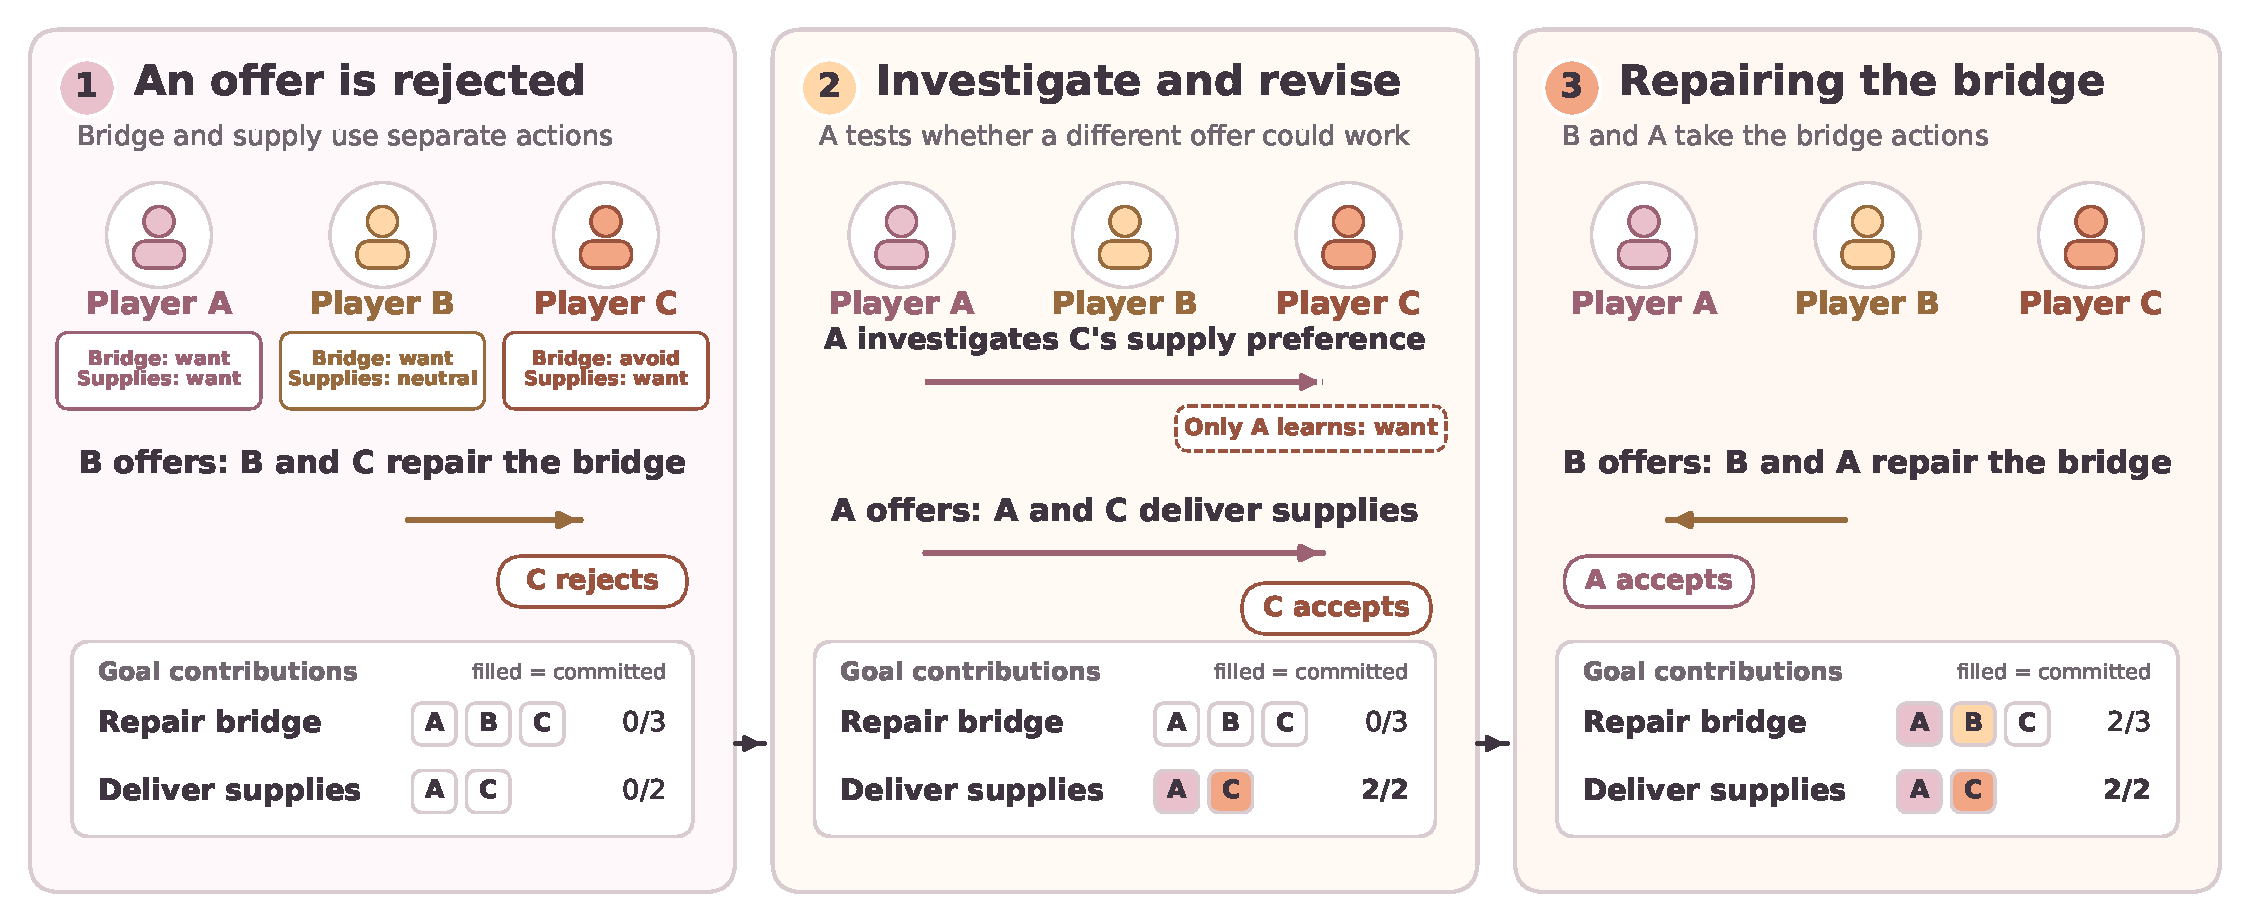
\includegraphics[width=\textwidth]{figures/game_flow.pdf}
\caption{An illustrative three-player trajectory before the personal
offer-quota extension. Filled letters indicate binding commitments, and
fractions show goal progress. Bridge and supply contributions are distinct
commitments. Investigation answers are private to the investigator, and
proposal opportunities follow the cyclic order B--A--C.}
\label{fig:game-flow}
\end{figure}

\section{Strategic Game Slices}
\label{sec:slices}
A strategic game slice begins at a decision context and evaluates a focal
player against fixed reference opponents. We distinguish three questions:
which actions have high terminal value (Q), how available information
supports those decisions (S), and how much value a target model loses (D).
The following definitions connect these quantities through a common
information structure and continuation model.

\subsection{Information Sets and the Reference Oracle}
The environment is a finite extensive-form game with hidden preference
types~\cite{harsanyi1967games}. Let $\theta$ be the joint type drawn from public prior $\mu_0$,
$h$ a public history, and $r_i$ player $i$'s private investigation record.
Its decision information is $I_i=(h,\theta_i,r_i)$, together with the
public instance. A behavioural strategy $\pi_i(a\mid I_i)$ assigns
probabilities to legal actions. Indistinguishable histories share the same
strategy. Players retain their observations and actions, giving the
perfect-recall structure underlying behavioural-strategy representations
of extensive games~\cite{kuhn1953extensive}.

The oracle selects a reference profile $\pi^{\mathrm{ref}}$ by searching
for mutually consistent best responses over complete contingent
strategies. For every player and positive-prior root type, certification
requires
\begin{equation}
 \max_{\pi_i\in\Pi_i}
 \E[U_i\mid\theta_i,\pi_i,\pi_{-i}^{\mathrm{ref}}]
 -\E[U_i\mid\theta_i,\pi^{\mathrm{ref}}]\leq\varepsilon,
 \label{eq:reference-certificate}
\end{equation}
where $\Pi_i$ is the set of legal information-respecting strategies.
This is a numerical Bayesian Nash best-response condition. Additional
checks enforce local optimality of supported actions and the response
objective in Section~\ref{sec:game}, using $\varepsilon=10^{-8}$ and tie
tolerance $10^{-9}$. These checks certify the selected numerical
reference; sequential equilibrium additionally requires belief consistency
at unreached information sets~\cite{kreps1982sequential}.

Behaviour provides evidence through the reference policy. For a candidate
world $\theta$ compatible with $I_i$, define its counterfactual prefix weight
\begin{equation}
 \lambda_{-i}(h,\theta)=\mu_0(\theta)
 \prod_{\substack{r\prec h:\,j_r\ne i}}
 \pi_{j_r}^{\mathrm{ref}}(a_r\mid I_{j_r}(\theta)).
 \label{eq:cf-weight}
\end{equation}
Here $r\prec h$ indexes observed decisions. When the compatible weights
have positive total mass, normalising them over worlds consistent with the
player's own type and private answers gives its belief
$b_i(\theta\mid I_i)$. Own past actions are excluded so that the
focal player can deviate from its reference strategy.

\subsection{Action Values and Best Responses}
After selecting the reference, opponents remain fixed during evaluation.
For a focal strategy $\pi_i$, write
\begin{equation}
 V_I(\pi_i)=\E[U_i\mid b_i(\cdot\mid I),\pi_i,
                              \pi_{-i}^{\mathrm{ref}}].
\end{equation}
The action value, optimal value, and regret are
\begin{align}
 Q_i(I,a)&=\max_{\pi_i\in\Pi_i:\,\pi_i(I)=a}V_I(\pi_i),
 \label{eq:q}\\
 V_i^*(I)&=\max_{a\in\mathcal L(I)}Q_i(I,a),\qquad
 R_i(I,a)=V_i^*(I)-Q_i(I,a).
 \label{eq:regret}
\end{align}
Thus Q forces the current action and optimises the focal player's
subsequent contingent behaviour to the native terminal state. It includes
later information acquisition, agreements, and responses. With opponents
fixed, evaluation becomes an information-constrained best-response problem
over the finite tree. Sequence-form
representations express strategies through realisation probabilities and
flow constraints~\cite{koller1996sequence}.

\subsection{Information Omission and Sensitivity}
To evaluate an observed item $e$, we remove access to one private answer
or one completed public proposal event. Rules, own preferences, current
commitments, pending offers, quotas, and legal actions remain visible.
Contexts with the same retained observations form an omission class
$\mathcal F_e$. We optimise a shared strategy $\pi_{-e}^*$ over this entry
forest, weighted by normalised counterfactual reach. From entry onward,
the strategy retains its remaining information and remembers new actions
and observations while the omitted item stays unavailable. Remaining
omission-policy ties are uniform after applying the response objective.

Let $\pi_I^*$ be optimal with all of the player's available observations.
The own-utility omission loss is
\begin{equation}
 S_e(I)=V_I(\pi_I^*)-V_I(\pi_{-e}^*).
 \label{eq:s}
\end{equation}
Both terms use the same true entry belief and opponents. The omitted
strategy is also available to the informed player, so $S_e(I)\geq0$.
Value-of-information methods similarly connect observations to achievable
decision quality~\cite{chen2017voi}. Here we evaluate the loss at an already realised
context rather than before acquiring the observation.

We distinguish subjective valuation after omission from evaluation at
the original context. The subjective
table $Q_e^-(\mathcal F_e,a)$ averages over the omission class and uses
omission-optimal continuation. The table $\widetilde Q_e(I,a)$ evaluates
that continuation after forcing $a$ at the true entry $I$. S therefore
compares policies under one belief, rather than maxima computed under
different beliefs.

Writing $p_e^-(a)=\pi_{-e}^*(a\mid\mathcal F_e)$ gives the exact decomposition
\begin{align}
 S_e(I)&=S_e^{\mathrm{current}}(I)+S_e^{\mathrm{future}}(I),
 \label{eq:s-decomp}\\
 S_e^{\mathrm{current}}(I)&=\sum_a p_e^-(a)R_i(I,a),\\
 S_e^{\mathrm{future}}(I)&=\sum_a p_e^-(a)
                      [Q_i(I,a)-\widetilde Q_e(I,a)].
\end{align}
The current term evaluates the chosen action with informed optimal
continuation, while the future term captures additional loss from continued
omission. It follows by substituting
$V_I(\pi_{-e}^*)=\sum_a p_e^-(a)\widetilde Q_e(I,a)$ into
Eq.~\ref{eq:s}. Consequently, an unchanged current choice can still conceal
later information loss.

\subsection{Action Profiles and Information Acquisition}
A scalar loss does not describe every change in decision structure.
We therefore also retain the relative regret vectors
$R_i(I,\cdot)$ and $R_e^-(\cdot)=\max_a Q_e^-(a)-Q_e^-(\cdot)$,
the optimal action sets, and canonical full/omitted action distributions.
The full distribution $p^+$ is uniform on actions that maximise own
utility after applying the response tie rule. Total variation, defined as
$\operatorname{TV}(p,q)=\tfrac12\sum_a|p(a)-q(a)|$, and Jensen--Shannon
divergence compare it with $p_e^-$.

These distributions follow the specified tie-breaking convention. Their
connection to own-utility loss is
\begin{equation}
 S_e^{\mathrm{current}}=(p^+-p_e^-)\cdot Q_i(I,\cdot)
 \leq[\max_a Q_i(I,a)-\min_a Q_i(I,a)]\,
       \operatorname{TV}(p^+,p_e^-).
 \label{eq:tv-bound}
\end{equation}
Thus switching between equally valuable actions can change the
distribution while leaving own loss zero. Relative regret also detects
changes among suboptimal actions when the optimal set stays unchanged.

Before investigation, let $\mathcal L_0(I_0)$ be the non-investigation
actions at entry $I_0$. The acquisition advantage is
\begin{equation}
 G_{j,g}(I_0)=Q_i(I_0,\mathrm{INVESTIGATE}(j,g))
             -\max_{a\in\mathcal L_0(I_0)}Q_i(I_0,a).
\end{equation}
This comparison includes the opportunity cost and all subsequent branches.

\subsection{Model Difficulty}
A slice $\sigma$ specifies a focal player, an entry distribution $\nu_\sigma$,
and a control/continuation contract. For the new terminal-control design,
the model controls the focal player from entry to terminal, while opponents
follow $\pi_{-i}^{\mathrm{ref}}$. If model $M$ induces policy $\pi_i^M$, define
\begin{align}
 V_\sigma^*&=\E_{I\sim\nu_\sigma}[V_i^*(I)],\\
 D_\sigma(M)&=V_\sigma^*
              -\E_{I\sim\nu_\sigma}[V_I(\pi_i^M)].
 \label{eq:d}
\end{align}
D is the expected terminal performance gap of the actual model under a
fixed prompt, tool interface, and decoding protocol. When all $N$ evaluation
rollouts complete with terminal utilities $u_i^{(m)}$, its estimate is
$\widehat D_\sigma=V_\sigma^*-N^{-1}\sum_{m=1}^N u_i^{(m)}$.

Q/S describe the strategic task; D measures the model's difficulty with
it. If all responses sampled at a decision receive the same reward, their
within-group task advantages are zero even when D is large. We therefore
measure sampling diversity and reward contrast alongside D.

\subsection{Selecting Slice Entrances}
\label{sec:slice-selection}
The selection procedure combines strategic coverage from Q/S
with measured model difficulty D. Each entrance is a player information
context rather than an individual hidden world.

\paragraph{Eligible contexts.}
We first retain entrances with a certified terminal reference and positive
counterfactual reach, then deduplicate identical observation contexts.
Different histories or beliefs remain distinct even when commitments and
budgets coincide. Each entrance retains its complete visible state,
reference identity, and terminal Q/S profile.

\paragraph{Strategic coverage.}
The profiles identify complementary demands. Positive S marks the value of
using an existing answer or historical observation. Its current/future
decomposition distinguishes immediate choice from later policy loss.
Zero-S contexts can still test valuation when information changes relative
regrets while preserving a common optimal action, or planning when a
myopic action is inferior under terminal Q. Information-acquisition
candidates are checked for both the query's Q advantage and the value of
receiving its answer compared with taking the same public query action
without answer access. This separates acquisition from public signalling.

\paragraph{Diversity and model difficulty.}
Candidate selection will cover different parents, goal structures, decision
phases, and remaining focal-decision lengths, protecting acquisition--use
chains without discarding useful single-decision tasks. Concentration by
parent and physical structure will be limited while preserving distinct
information contexts. We will construct 800 candidates including a reserved
validation portion. Under a fixed prompt, decoding protocol, and focal
control to terminal, repeated model rollouts on the training candidates
will estimate D and sampled action/reward diversity. These measurements
will guide selection of 100 training slices within the coverage design,
rather than ranking all entrances by S, Q span, or distribution distance.

\section{Model Diagnosis}
\label{sec:diagnosis}
We separate inference from planning at an explicit judgment--action
interface. Inference maps observed evidence to a judgment about a partner's
hidden preference; planning maps the current decision state and a supplied
judgment to an action. Independent calls let us replace the inference
output while holding the planning task fixed.

\subsection{Task Separation and Oracle Labels}
The diagnostic contains 22 two-player cases across seven game structures.
Each queries one hidden partner--goal preference
$z\in\{\mathrm{want},\mathrm{neutral},\mathrm{avoid}\}$. The evidence
comprises six direct investigation answers, six single-choice elimination
cases, six ambiguous single-choice cases, and four multi-step updates.
For case $c$, the reference oracle conditions on the public prior, own
preferences, private answers, and observed partner choices to obtain
$p_c^*(z)$.

The inference label $J_c^*=(\mathcal S_c^*,m_c^*)$ contains the support
$\mathcal S_c^*=\{z:p_c^*(z)>0\}$ and a favoured preference $m_c^*$.
The latter is the highest-probability value only if its probability exceeds
the runner-up by more than $0.1$; otherwise, it is undetermined. The model
receives the original visible evidence and submits the corresponding
support and favoured value through a belief-submission tool. These labels
supervise what the evidence supports, rather than requiring the model to
guess the realised hidden value.

Planning receives the rules, goal requirements, known preferences, current
commitments, pending offer, schedule position, remaining investigation
budget, and legal action tools. Behavioural history and the queried
private answer are replaced by the supplied qualitative judgment. Neither
numerical posterior probabilities nor oracle action values are disclosed.
The model must select an action using this judgment and the retained
physical state.

\begin{table}[tb]
\centering\small
\caption{Four diagnostic calls at each matched decision. Each call is a
fresh request. The two planning calls differ only in the supplied judgment.}
\label{tab:diagnostic-design}
\begin{tabularx}{\textwidth}{p{28mm}YY}
\toprule
Condition & Input & Scored output\\
\midrule
Inference & Original state and visible evidence & Preference judgment
$\widehat J_c$\\
Direct action & Original state and visible evidence & Native game action\\
Plan: model & History-free state and $\widehat J_c$ & Native game action\\
Plan: oracle & Same history-free state and $J_c^*$ & Native game action\\
\bottomrule
\end{tabularx}
\end{table}

The direct-action call measures performance without an explicit supplied
inference. For the paired planning calls in
Table~\ref{tab:diagnostic-design}, tools, decoding settings, and request
seed are identical. Removing behavioural evidence prevents planning from
simply reconstructing the original inference, and replacing only the judgment
measures its effect on the selected action.

\subsection{Supervision and Protocol Validation}
Exact rational checks verify that all posteriors compatible with the
oracle judgment share the same optimal-action set. The scorer's
tolerance-based acceptable set is checked over these regions as well.
We also recompute legal
actions and continuation payoffs from the history-free state to verify
that removing history preserves the planning problem.

Inference correctness requires both submitted label components to match
$J_c^*$. Action correctness uses the certified acceptable-action set,
with an own-utility tolerance of $0.1$ and the diagnostic's response
social-tie tolerance of $0.1$. These are historical scoring tolerances,
separate from the reference solver's numerical tolerance. The same label
format is used for the inference and conditional-planning training
objectives described in Section~\ref{sec:training-testing}.

To measure consequences, let $W_c(a,z)$ be the diagnostic's fixed
per-preference terminal continuation payoff for action $a$, and define
\begin{align}
 v_c(a)&=\sum_z p_c^*(z)W_c(a,z),\\
 \operatorname{Reg}_c(a)&=\max_b v_c(b)-v_c(a),\\
 \Delta_c&=v_c\bigl(\widehat a_c(J_c^*)\bigr)
           -v_c\bigl(\widehat a_c(\widehat J_c)\bigr).
 \label{eq:diagnostic-intervention}
\end{align}
Here $\widehat a_c(J)$ denotes the model's action given judgment $J$.
Both actions are evaluated under the same oracle posterior and the
diagnostic's fixed reference continuation, rather than rescored under their different
supplied judgments. Positive $\Delta_c$ indicates that judgment replacement
improves the decision.

The suite includes nine repair-sensitive cases, where an alternative
preference can require an incompatible acceptable action, and thirteen
action controls. All four multi-step cases are controls with a common
acceptable action across preferences. This distinction identifies cases
where judgment replacement can require an action change.

\subsection{Diagnostic Results}
We evaluate Qwen3-4B-Instruct-2507~\cite{qwen2025instruct2507} once per case at temperature
zero, with a 4,096-token output limit. One model-judgment planning response
has a format failure. It counts as incorrect for accuracy and is excluded
from paired utility comparisons, leaving 21 valid pairs.

\begin{table}[tb]
\centering\small
\caption{Base-model diagnostic accuracy. Joint inference requires both
posterior support and the most likely preference to match the oracle.}
\label{tab:diagnosis}
\begin{tabular}{lrrrr}
\toprule
Evidence & Inference & Direct & Plan: model & Plan: oracle\\
\midrule
Direct investigation answer & 6/6 & 2/6 & 3/6 & 3/6\\
Single-choice elimination & 0/6 & 3/6 & 2/6 & 3/6\\
Ambiguous single choice & 5/6 & 2/6 & 2/6 & 2/6\\
Multi-step update & 0/4 & 4/4 & 4/4 & 3/4\\
\midrule
Total & 11/22 & 11/22 & 11/22 & 11/22\\
\bottomrule
\end{tabular}
\end{table}

Table~\ref{tab:diagnosis} reveals distinct inference and planning failures.
The model recovers all six directly revealed preferences, yet planning
with oracle judgments succeeds in only three of these six cases. Across
all cases, each action condition scores 11/22. Among ten valid pairs with
incorrect initial judgments, replacement improves utility in three,
leaves it unchanged in six, and reduces it in one. Across all 21 valid
pairs, mean regret falls from $0.684$ to $0.541$ despite unchanged aggregate
accuracy. Supplying a correct inference can help, but does not reliably
resolve the remaining planning difficulty.

\section{Training and Testing}
\label{sec:training-testing}
The diagnostic results motivate training preference inference and
conditional planning alongside direct action selection. We evaluate the
trained checkpoints on
private-calendar coordination, which uses different actions and interaction
mechanics from the negotiation game.

\subsection{Training Objectives and Comparisons}
All training variants use Qwen3-4B-Instruct-2507 as their base model.
In direct-action training, oracle labels score the model's proposed actions. The
action-and-planning variant additionally trains decisions conditioned on
oracle preference judgments, and joint training adds explicit preference
inference. These tasks update a shared model through grouped reinforcement
learning~\cite{shao2024deepseekmath}. At test time, the model selects actions
from its observations without receiving oracle judgments.

Complete-game self-play provides a comparison in which players learn from
their own terminal utilities through full interactions. We also evaluate
the unchanged base model. Table~\ref{tab:transfer} denotes direct-action,
action-and-planning, and joint training by \textsc{GameSlice-A},
\textsc{GameSlice-AP}, and \textsc{GameSlice-Joint}, respectively.

\subsection{Transfer to Sequential Calendar Coordination}
The preliminary transfer experiment uses a local sequential adaptation
of CalBench~\cite{zou2026calbench}. Four agents coordinate three meetings in each
of 24 fixed scenarios. Agents observe private calendars and communicate
to establish common meeting slots while preserving earlier commitments.
Every player in a team uses the same checkpoint. We report retained
meetings out of 72 and complete games out of 24. Excess cost is computed
by subtracting the minimum feasible team cost from the realised cost,
dividing by four, and averaging over complete games. Communication and
burden imbalance are averaged over agents and games. Communication counts
messages per round-level scheduling success, with a minimum denominator
of one; imbalance measures deviations in excess rescheduling burdens.
We additionally compare
Qwen3-4B (thinking), MARSHAL Generalist, and Social-R1-4B~\cite{wu2026socialr1}.

\begin{table}[tb]
\caption{CalBench transfer on 24 frozen sequential games. Meetings count
final retained meetings; excess cost is per agent and conditional on full-game
success. Communication and imbalance average native per-agent values over all
games.}
\label{tab:transfer}
\centering\small
\setlength{\tabcolsep}{4pt}
\begin{tabular}{lccccc}
\hline
Model & Meetings $\uparrow$ & Full games $\uparrow$ & Cost $\downarrow$ & Comm. $\downarrow$ & Imbalance $\downarrow$ \\
\hline
Baseline & 37 & 5 & 0.100 & 5.663 & 0.443 \\
Self-play & 37 & 6 & 0.625 & 5.181 & 0.755 \\
GameSlice-A & 38 & 8 & 0.688 & 5.003 & 0.490 \\
GameSlice-AP & 44 & 10 & 0.075 & 4.760 & 0.432 \\
GameSlice-Joint & 47 & 9 & 0.194 & 4.714 & 0.292 \\
\hline
Qwen3-4B (thinking) & 42 & 7 & 0.571 & 4.828 & 0.557 \\
MARSHAL Generalist & 37 & 6 & 1.333 & 4.429 & 0.875 \\
Social-R1-4B & 39 & 5 & 1.100 & 4.554 & 0.901 \\
\hline
\end{tabular}
\end{table}

\textsc{GameSlice-Joint} retains ten more meetings than the baseline and
self-play and has lower communication overhead and burden imbalance.
\textsc{GameSlice-AP} completes the most full games and has the lowest
conditional excess cost (Table~\ref{tab:transfer}). Cost averages cover
different successful subsets for different models. These preliminary
comparisons motivate further testing of conditional-planning supervision
for transfer. Since training exposure and inference settings differ across
the runs, the next phase will compare matched budgets over repeated runs.

\section{Discussion}
\label{sec:discussion}
\paragraph{Beyond preference inference.}
Our games locate uncertainty primarily in partners' preferences. Real
coordination also requires reasoning about what others have observed and
what they believe others know, as explored in recent multi-agent theory-of-mind
work \citep{ys2026sotopiatom,mu2026adaptive,cross2025hypothetical}. These hidden
states belong within inference, but introduce a further challenge: the same
refusal may reflect conflicting preferences or missing information, calling
for different responses. Future game slices could vary knowledge and
preferences independently, testing whether agents distinguish these causes
and choose when to clarify or disclose information. The
key question is which distinctions in a partner's mental state are necessary
for a good decision.

\paragraph{Coverage and interaction.}
Game slices let us select strategically consequential decisions and verify
their supervision. Self-play provides coherent interaction trajectories, but
visits states according to the current policies and may encounter important
decisions infrequently. This motivates targeting such decisions explicitly,
consistent with work on subgame curricula \citep{chen2024subgame}. A possible next step is to combine
the two: use self-play to identify recurring failures, construct and solve
slices around those decisions, and return to complete games to evaluate the
learned behaviour. This would test whether targeted practice can repair local
weaknesses while preserving effective coordination over an entire interaction.

\paragraph{Inference under unfamiliar partner policies.}
Our oracle assumes a fixed partner policy, while self-play primarily exposes
a model to copies of its evolving policy. Yet the meaning of an observed
action depends on how the partner chooses: a rejection that rules out a
preference under one policy may be compatible with it under another.
Cross-partner coordination research motivates training with diverse partner
populations \citep{hu2020otherplay,strouse2021collaborating}. For game slices,
this means varying planning horizons, tie-breaking rules, or action noise and
recomputing labels under each behavioural model. Evaluation on held-out
policy families would test whether agents can interpret unfamiliar behaviour
and adapt their plans beyond the assumptions of a single oracle.

\section{Research Plan for the Next Semester}
\label{sec:future-plan}
Building on the selection procedure in Section~\ref{sec:slice-selection}
and the discussion of partner generalisation, next semester's work will
compare prompt systems with post-training and identify the capabilities
responsible for improved coordination.

\subsection{Prompt Systems versus Post-Training}
We will compare modifying the inference-time prompt system with updating
model parameters through slice-based post-training. The prompt system will
structure evidence tracking, judgments about partners, and action planning
while keeping model weights fixed. A factorial comparison will evaluate
four conditions: the base model with the original prompt, the base model
with the structured prompt system, the post-trained model with the original
prompt, and the post-trained model with the structured prompt system.
All conditions will receive the same task information and action tools.

This design tests whether prompting and post-training provide independent,
complementary, or substitutable benefits. We will compare negotiation
regret and calendar coordination at matched inference budgets, recording
generated tokens, model calls, and latency. Training cost will be reported
separately to assess the trade-off between one-time parameter updates and
repeated inference overhead. Applying the same prompt system to both
checkpoints will also test whether training improves the use of explicit
reasoning support. Prompt variants will be selected on validation tasks
before evaluation on the test set.

\subsection{Which Capabilities Improve and Transfer?}
We will examine improvements in four capabilities: maintaining and updating
beliefs from interaction history; identifying useful information to seek
or disclose; planning actions using inferred constraints; and revising
plans while preserving commitments across participants and turns. Matched
decision probes will compare base and post-trained models on the same
visible contexts. The inference/planning intervention in
Section~\ref{sec:diagnosis} will test whether gains remain when both models
receive the same correct judgment. Training-objective ablations will
examine the contributions of inference and conditional-planning supervision.

In calendar coordination, we will track whether agents incorporate new
constraints, check proposed times with affected participants, and repair
conflicts while preserving existing meetings. Controlled scenarios and
corrected-judgment interventions will link these process measures to final
meeting retention and cost, connecting decision-level gains to complete
coordination outcomes.

\clearpage
\begingroup
\small\setstretch{1.0}\raggedright
\setlength{\parskip}{0pt}
\bibliographystyle{unsrtnat}
\bibliography{references,ca_report_additional}
\endgroup
\end{document}
